% Options for packages loaded elsewhere
\PassOptionsToPackage{unicode}{hyperref}
\PassOptionsToPackage{hyphens}{url}
%
\documentclass[
]{article}
\usepackage{lmodern}
\usepackage{amssymb,amsmath}
\usepackage{ifxetex,ifluatex}
\ifnum 0\ifxetex 1\fi\ifluatex 1\fi=0 % if pdftex
  \usepackage[T1]{fontenc}
  \usepackage[utf8]{inputenc}
  \usepackage{textcomp} % provide euro and other symbols
\else % if luatex or xetex
  \usepackage{unicode-math}
  \defaultfontfeatures{Scale=MatchLowercase}
  \defaultfontfeatures[\rmfamily]{Ligatures=TeX,Scale=1}
\fi
% Use upquote if available, for straight quotes in verbatim environments
\IfFileExists{upquote.sty}{\usepackage{upquote}}{}
\IfFileExists{microtype.sty}{% use microtype if available
  \usepackage[]{microtype}
  \UseMicrotypeSet[protrusion]{basicmath} % disable protrusion for tt fonts
}{}
\makeatletter
\@ifundefined{KOMAClassName}{% if non-KOMA class
  \IfFileExists{parskip.sty}{%
    \usepackage{parskip}
  }{% else
    \setlength{\parindent}{0pt}
    \setlength{\parskip}{6pt plus 2pt minus 1pt}}
}{% if KOMA class
  \KOMAoptions{parskip=half}}
\makeatother
\usepackage{xcolor}
\IfFileExists{xurl.sty}{\usepackage{xurl}}{} % add URL line breaks if available
\IfFileExists{bookmark.sty}{\usepackage{bookmark}}{\usepackage{hyperref}}
\hypersetup{
  hidelinks,
  pdfcreator={LaTeX via pandoc}}
\urlstyle{same} % disable monospaced font for URLs
\usepackage{color}
\usepackage{fancyvrb}
\newcommand{\VerbBar}{|}
\newcommand{\VERB}{\Verb[commandchars=\\\{\}]}
\DefineVerbatimEnvironment{Highlighting}{Verbatim}{commandchars=\\\{\}}
% Add ',fontsize=\small' for more characters per line
\newenvironment{Shaded}{}{}
\newcommand{\AlertTok}[1]{\textcolor[rgb]{1.00,0.00,0.00}{\textbf{#1}}}
\newcommand{\AnnotationTok}[1]{\textcolor[rgb]{0.38,0.63,0.69}{\textbf{\textit{#1}}}}
\newcommand{\AttributeTok}[1]{\textcolor[rgb]{0.49,0.56,0.16}{#1}}
\newcommand{\BaseNTok}[1]{\textcolor[rgb]{0.25,0.63,0.44}{#1}}
\newcommand{\BuiltInTok}[1]{#1}
\newcommand{\CharTok}[1]{\textcolor[rgb]{0.25,0.44,0.63}{#1}}
\newcommand{\CommentTok}[1]{\textcolor[rgb]{0.38,0.63,0.69}{\textit{#1}}}
\newcommand{\CommentVarTok}[1]{\textcolor[rgb]{0.38,0.63,0.69}{\textbf{\textit{#1}}}}
\newcommand{\ConstantTok}[1]{\textcolor[rgb]{0.53,0.00,0.00}{#1}}
\newcommand{\ControlFlowTok}[1]{\textcolor[rgb]{0.00,0.44,0.13}{\textbf{#1}}}
\newcommand{\DataTypeTok}[1]{\textcolor[rgb]{0.56,0.13,0.00}{#1}}
\newcommand{\DecValTok}[1]{\textcolor[rgb]{0.25,0.63,0.44}{#1}}
\newcommand{\DocumentationTok}[1]{\textcolor[rgb]{0.73,0.13,0.13}{\textit{#1}}}
\newcommand{\ErrorTok}[1]{\textcolor[rgb]{1.00,0.00,0.00}{\textbf{#1}}}
\newcommand{\ExtensionTok}[1]{#1}
\newcommand{\FloatTok}[1]{\textcolor[rgb]{0.25,0.63,0.44}{#1}}
\newcommand{\FunctionTok}[1]{\textcolor[rgb]{0.02,0.16,0.49}{#1}}
\newcommand{\ImportTok}[1]{#1}
\newcommand{\InformationTok}[1]{\textcolor[rgb]{0.38,0.63,0.69}{\textbf{\textit{#1}}}}
\newcommand{\KeywordTok}[1]{\textcolor[rgb]{0.00,0.44,0.13}{\textbf{#1}}}
\newcommand{\NormalTok}[1]{#1}
\newcommand{\OperatorTok}[1]{\textcolor[rgb]{0.40,0.40,0.40}{#1}}
\newcommand{\OtherTok}[1]{\textcolor[rgb]{0.00,0.44,0.13}{#1}}
\newcommand{\PreprocessorTok}[1]{\textcolor[rgb]{0.74,0.48,0.00}{#1}}
\newcommand{\RegionMarkerTok}[1]{#1}
\newcommand{\SpecialCharTok}[1]{\textcolor[rgb]{0.25,0.44,0.63}{#1}}
\newcommand{\SpecialStringTok}[1]{\textcolor[rgb]{0.73,0.40,0.53}{#1}}
\newcommand{\StringTok}[1]{\textcolor[rgb]{0.25,0.44,0.63}{#1}}
\newcommand{\VariableTok}[1]{\textcolor[rgb]{0.10,0.09,0.49}{#1}}
\newcommand{\VerbatimStringTok}[1]{\textcolor[rgb]{0.25,0.44,0.63}{#1}}
\newcommand{\WarningTok}[1]{\textcolor[rgb]{0.38,0.63,0.69}{\textbf{\textit{#1}}}}
\usepackage{longtable,booktabs}
% Correct order of tables after \paragraph or \subparagraph
\usepackage{etoolbox}
\makeatletter
\patchcmd\longtable{\par}{\if@noskipsec\mbox{}\fi\par}{}{}
\makeatother
% Allow footnotes in longtable head/foot
\IfFileExists{footnotehyper.sty}{\usepackage{footnotehyper}}{\usepackage{footnote}}
\makesavenoteenv{longtable}
\usepackage{graphicx}
\makeatletter
\def\maxwidth{\ifdim\Gin@nat@width>\linewidth\linewidth\else\Gin@nat@width\fi}
\def\maxheight{\ifdim\Gin@nat@height>\textheight\textheight\else\Gin@nat@height\fi}
\makeatother
% Scale images if necessary, so that they will not overflow the page
% margins by default, and it is still possible to overwrite the defaults
% using explicit options in \includegraphics[width, height, ...]{}
\setkeys{Gin}{width=\maxwidth,height=\maxheight,keepaspectratio}
% Set default figure placement to htbp
\makeatletter
\def\fps@figure{htbp}
\makeatother
\setlength{\emergencystretch}{3em} % prevent overfull lines
\providecommand{\tightlist}{%
  \setlength{\itemsep}{0pt}\setlength{\parskip}{0pt}}
\setcounter{secnumdepth}{-\maxdimen} % remove section numbering

\author{}
\date{}

\begin{document}

TD n°15 : Structures de données - Les Dictionnaires

Thème 1 : Structures de données

COURS et EXERCICES

\begin{figure}
\centering
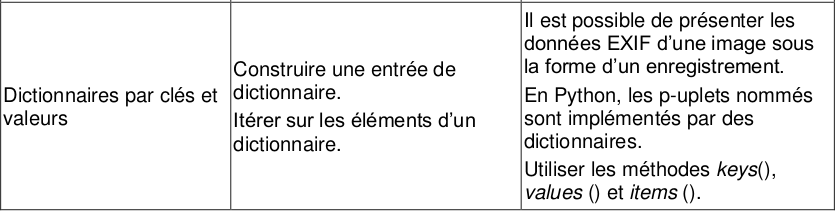
\includegraphics{data/BO.png}
\caption{BO.png}
\end{figure}

\hypertarget{introduction-nuxe9cessituxe9-dun-dictionnaire}{%
\section{Introduction : nécessité d'un
dictionnaire}\label{introduction-nuxe9cessituxe9-dun-dictionnaire}}

Prenons l'exemple d'un répertoire téléhonique. Nous pouvons le mémoriser
simplement comme un tableau (ou liste) de tableaux
\texttt{{[}nom,numéro{]}}

\begin{Shaded}
\begin{Highlighting}[]
\NormalTok{liste\_tel }\OperatorTok{=}\NormalTok{ [[}\StringTok{"Paul"}\NormalTok{, }\StringTok{\textquotesingle{}0650523454\textquotesingle{}}\NormalTok{],}
\NormalTok{             [}\StringTok{"Emile"}\NormalTok{, }\StringTok{\textquotesingle{}0684515345\textquotesingle{}}\NormalTok{],}
\NormalTok{             [}\StringTok{"Victor"}\NormalTok{, }\StringTok{\textquotesingle{}0651355186\textquotesingle{}}\NormalTok{],}
\NormalTok{             [}\StringTok{"Rose"}\NormalTok{, }\StringTok{\textquotesingle{}0611245678\textquotesingle{}}\NormalTok{],}
\NormalTok{             [}\StringTok{"Hélène"}\NormalTok{, }\StringTok{\textquotesingle{}0774845432\textquotesingle{}}\NormalTok{]]}
\end{Highlighting}
\end{Shaded}

Si nous voulons appeler \emph{Rose}, nous avons deux possibilités avec
un tel tableau : * soit il faut savoir que les informations la
concernant sont dans le quatrième élément de la liste (ce qui ne semble
pas très pratique et réaliste)

\begin{Shaded}
\begin{Highlighting}[]
\BuiltInTok{print}\NormalTok{(liste\_tel[}\DecValTok{3}\NormalTok{][}\DecValTok{1}\NormalTok{]) }\CommentTok{\# il faut savoir que l\textquotesingle{}index de Rose est 3}
\end{Highlighting}
\end{Shaded}

\begin{itemize}
\tightlist
\item
  soit nous cherchons dans le tableau en partant du premier élément de
  la liste jusqu'à ce que nous trouvions \emph{Rose} (ce qui revient à
  feuilleter son répertoire) : cela nécessite d'utiliser une boucle pour
  parcourir le tableau.
\end{itemize}

\begin{Shaded}
\begin{Highlighting}[]
\ControlFlowTok{for}\NormalTok{ element }\KeywordTok{in}\NormalTok{ liste\_tel:}
    \ControlFlowTok{if}\NormalTok{ element[}\DecValTok{0}\NormalTok{] }\OperatorTok{==} \StringTok{\textquotesingle{}Rose\textquotesingle{}}\NormalTok{:}
        \BuiltInTok{print}\NormalTok{(element[}\DecValTok{1}\NormalTok{])}
\end{Highlighting}
\end{Shaded}

Vous conviendrez que \textbf{ce n'est pas pratique} pour accéder à son
numéro de téléphone.\\
De même, la modification ou l'ajout d'un information nécessiterait de
devoir feuilleter tout le répertoire. Il semblerait plus pratique
d'associer un nom à un numéro, autrement dit d'associer à une
\textbf{information} à une \textbf{clé}.

C'est ce que les dictionnaires permettent !

\hypertarget{ii.-les-dictionnaires-en-python}{%
\section{II. Les dictionnaires en
Python}\label{ii.-les-dictionnaires-en-python}}

\hypertarget{duxe9finitions-et-premiers-exemples}{%
\subsection{Définitions et premiers
exemples}\label{duxe9finitions-et-premiers-exemples}}

💜 Un dictionnaire, de \textbf{type dict} en Python, est un ensemble
\textbf{non ordonné} de paires (clé, valeur) avec un accès très rapide à
la valeur à partir de la clé.

C'est un type de conteneur comme les list et les tuple mais ce n'est pas
une séquence. Au sens où les valeurs des tableaux ne sont pas indexés
par des entiers.

Dans un dictionnaire, \textbf{chaque élément est accessible par une clé}
qui n'est plus forcément un nombre, une chaine de caractère, un nombre,
ou autre chose, peut être une clé.

\textbf{🖋 Exemple n°1 :}

Reprenons la problématique de départ : un répertoire téléhonique.\\
Nous pouvons le mémoriser comme un dictionnaire
\texttt{{[}nom:numéro{]}}

\begin{Shaded}
\begin{Highlighting}[]
\OperatorTok{\textgreater{}\textgreater{}\textgreater{}}\NormalTok{ repertoire }\OperatorTok{=}\NormalTok{ \{}\StringTok{"Paul"}\NormalTok{: }\StringTok{\textquotesingle{}0650523454\textquotesingle{}}\NormalTok{,}\StringTok{"Emile"}\NormalTok{ : }\StringTok{\textquotesingle{}0684515345\textquotesingle{}}\NormalTok{,}\StringTok{"Victor"}\NormalTok{:}\StringTok{\textquotesingle{}0651355186\textquotesingle{}}\NormalTok{,}\StringTok{"Rose"}\NormalTok{: }\StringTok{\textquotesingle{}0611245678\textquotesingle{}}\NormalTok{,}\StringTok{"Hélène"}\NormalTok{: }\StringTok{\textquotesingle{}0774845432\textquotesingle{}}\NormalTok{\}}
\end{Highlighting}
\end{Shaded}

\begin{itemize}
\tightlist
\item
  L'accès à Rose se fera par :
\end{itemize}

\begin{Shaded}
\begin{Highlighting}[]
\OperatorTok{\textgreater{}\textgreater{}\textgreater{}}\NormalTok{ repertoire[}\StringTok{"Rose"}\NormalTok{]}
\CommentTok{\textquotesingle{}0611245678\textquotesingle{}}
\end{Highlighting}
\end{Shaded}

\begin{itemize}
\item
  On dit que \texttt{"Rose"} est \textbf{la clé} et que `0611245678' est
  \textbf{la valeur} associée à la clé.
\item
  Un dictionnaire est un ensemble clés / valeurs.
\end{itemize}

\textbf{🖋 A vous n°1 :}

Imaginons que je fasse l'inventaire de mon dressing :

\begin{longtable}[]{@{}cc@{}}
\toprule
habits & quantité\tabularnewline
\midrule
\endhead
pantalons & 3\tabularnewline
pulls & 4\tabularnewline
tee-shirts & 8\tabularnewline
\bottomrule
\end{longtable}

!!! fabquestion ``Question 1 :'' Créer le dictionnaire représentant mon
dressing.

!!! fabquestion ``Question 2 :'' Donner le script permettant d'accéder
au nombre de pulls présent dans mon dressing.

\hypertarget{duxe9finitions-et-propriuxe9tuxe9s-dun-dictionnaire}{%
\subsection{Définitions et propriétés d'un
dictionnaire}\label{duxe9finitions-et-propriuxe9tuxe9s-dun-dictionnaire}}

\hypertarget{duxe9finitions}{%
\subsubsection{Définitions}\label{duxe9finitions}}

!!! savoir ``📘 Définition''\\
Un dictionnaire est une donnée composite qui \textbf{n'est pas ordonnée}
(à la différence des listes !)\\
Il fonctionne par un système de \texttt{clé:valeur}.\\
Les clés, comme les valeurs, peuvent être de types différents.\\
Un dictionnaire est délimité par des accolades.

\emph{Rappel :}

\begin{itemize}
\tightlist
\item
  crochets \texttt{{[}\ {]}} -\textgreater{} listes
\item
  parenthèses \texttt{(\ )} -\textgreater{} tuples
\item
  \textbf{accolades \texttt{\{\ \}} -\textgreater{} dictionnaires}
\end{itemize}

\hypertarget{muxe9thodes-.keys-et-.values}{%
\subsubsection{\texorpdfstring{Méthodes \texttt{.keys()} et
\texttt{.values()}}{Méthodes .keys() et .values()}}\label{muxe9thodes-.keys-et-.values}}

\textbf{📎 Exemple n°2 :}

\begin{itemize}
\tightlist
\item
  Pour lister les clés d'un dictionnaire :
\end{itemize}

\begin{Shaded}
\begin{Highlighting}[]
\OperatorTok{\textgreater{}\textgreater{}\textgreater{}}\NormalTok{ repertoire.keys()}
\NormalTok{dict\_keys([}\StringTok{"Paul"}\NormalTok{,}\StringTok{"Emile"}\NormalTok{,}\StringTok{"Victor"}\NormalTok{,}\StringTok{"Rose"}\NormalTok{,}\StringTok{"Hélène"}\NormalTok{])}
\end{Highlighting}
\end{Shaded}

\begin{itemize}
\tightlist
\item
  Pour lister les valeurs d'un dictionnaire :
\end{itemize}

\begin{Shaded}
\begin{Highlighting}[]
\OperatorTok{\textgreater{}\textgreater{}\textgreater{}}\NormalTok{ repertoire.values()}
\NormalTok{dict\_values(}\StringTok{\textquotesingle{}0650523454\textquotesingle{}}\NormalTok{,}\StringTok{\textquotesingle{}0684515345\textquotesingle{}}\NormalTok{,}\StringTok{\textquotesingle{}0651355186\textquotesingle{}}\NormalTok{,}\StringTok{\textquotesingle{}0611245678\textquotesingle{}}\NormalTok{,}\StringTok{\textquotesingle{}0774845432\textquotesingle{}}\NormalTok{)}
\end{Highlighting}
\end{Shaded}

🖋 \textbf{A vous n°2 :}

!!! fabquestion ``Question 1''

\begin{verbatim}
- Lister les clés du dictionnaire dressing.

[!comment]: <> (```python)
[!comment]: <> (>>> dressing.keys())
[!comment]: <> (dict_keys(['pantalons', 'pulls', 'tee-shirts']))
[!comment]: <> (```)
\end{verbatim}

!!! fabquestion ``Question 2'' Lister les valeurs du dictionnaire
dressing.

\begin{verbatim}
[!comment]: <> (```python)
[!comment]: <> (>>> dressing.values())
[!comment]: <> (dict_values([3, 4, 8]))
[!comment]: <> (```)
\end{verbatim}

\hypertarget{parcours-dun-dictionnaire}{%
\subsubsection{Parcours d'un dictionnaire
:}\label{parcours-dun-dictionnaire}}

Il est possible de parcourir un dictionnaire de trois manières :

\begin{itemize}
\tightlist
\item
  parcourir l'ensemble des \textbf{clés} avec la méthode \texttt{keys()}
  ;
\item
  parcourir l'ensemble des \textbf{valeurs} avec la méthode
  \texttt{values()} ;
\item
  parcourir l'ensemble des \textbf{paires clés-valeurs} avec la méthode
  \texttt{items()}.
\end{itemize}

On peut itérer sur un dictionnaire grâce à l'une de ces méthodes.

\textbf{📎 Exemple n°3 : par les clés (idem tableau)}

\begin{Shaded}
\begin{Highlighting}[]
\OperatorTok{\textgreater{}\textgreater{}\textgreater{}} \ControlFlowTok{for}\NormalTok{ nom }\KeywordTok{in}\NormalTok{ repertoire:}
       \BuiltInTok{print}\NormalTok{(repertoire[nom])}
\NormalTok{0650523454}
\NormalTok{0684515345}
\NormalTok{0651355186}
\NormalTok{0611245678}
\NormalTok{0774845432}
\end{Highlighting}
\end{Shaded}

Par cette méthode, on obtient les valeurs associées aux clés.

\textbf{📎 Exemple n°4 : par les }clés** avec la méthode
\texttt{keys()}.**

\begin{Shaded}
\begin{Highlighting}[]
\OperatorTok{\textgreater{}\textgreater{}\textgreater{}} \ControlFlowTok{for}\NormalTok{ nom }\KeywordTok{in}\NormalTok{ repertoire.keys():}
        \BuiltInTok{print}\NormalTok{(nom)}
\NormalTok{Paul}
\NormalTok{Emile}
\NormalTok{Victor}
\NormalTok{Rose}
\NormalTok{Hélène}
\end{Highlighting}
\end{Shaded}

Par cette méthodes, on extrait les clés.

ou

\begin{Shaded}
\begin{Highlighting}[]
\OperatorTok{\textgreater{}\textgreater{}\textgreater{}} \ControlFlowTok{for}\NormalTok{ nom }\KeywordTok{in}\NormalTok{ repertoire.keys():}
        \BuiltInTok{print}\NormalTok{(repertoire[nom])}
\NormalTok{0650523454}
\NormalTok{0684515345}
\NormalTok{0651355186}
\NormalTok{0611245678}
\NormalTok{0774845432}
\end{Highlighting}
\end{Shaded}

Par cette méthode, on obtient les valeurs associées aux clés.

\textbf{📎 Exemple n°5 : par les }valeurs** avec la méthode
\texttt{values()}.**

\begin{Shaded}
\begin{Highlighting}[]
\OperatorTok{\textgreater{}\textgreater{}\textgreater{}} \ControlFlowTok{for}\NormalTok{ numero }\KeywordTok{in}\NormalTok{ repertoire.values():}
        \BuiltInTok{print}\NormalTok{(numero)}
\NormalTok{0650523454}
\NormalTok{0684515345}
\NormalTok{0651355186}
\NormalTok{0611245678}
\NormalTok{0774845432}
\end{Highlighting}
\end{Shaded}

Par cette méthodes, on extrait les valeurs présentes dans le
dictionnaires.

\textbf{📎 Exemple n°6 : par les }clés et les valeurs** avec la méthode
\texttt{items()}.**

\begin{Shaded}
\begin{Highlighting}[]
\OperatorTok{\textgreater{}\textgreater{}\textgreater{}} \ControlFlowTok{for}\NormalTok{ cle,valeur }\KeywordTok{in}\NormalTok{ repertoire.items():}
        \BuiltInTok{print}\NormalTok{(cle,valeur)}
\NormalTok{Paul 0650523454}
\NormalTok{Emile 0684515345}
\NormalTok{Victor 0651355186}
\NormalTok{Rose 0611245678}
\NormalTok{Hélène 0774845432}
\end{Highlighting}
\end{Shaded}

Par cette méthodes, on extrait les valeurs et les clés du dictionnaires.

\textbf{📎 Exemple n°7 : un dictionnaire dans un dictionnaire.}

\begin{Shaded}
\begin{Highlighting}[]
\NormalTok{sportifs }\OperatorTok{=}\NormalTok{ \{}\StringTok{"Mike"}\NormalTok{: \{}\StringTok{"taille"}\NormalTok{: }\FloatTok{1.75}\NormalTok{,}\StringTok{"poids"}\NormalTok{: }\DecValTok{68}\NormalTok{\}, }\StringTok{"John"}\NormalTok{: \{}\StringTok{"taille"}\NormalTok{: }\FloatTok{1.89}\NormalTok{,}\StringTok{"poids"}\NormalTok{: }\DecValTok{93}\NormalTok{\}, }\StringTok{"Kate"}\NormalTok{: \{}\StringTok{"taille"}\NormalTok{: }\FloatTok{1.67}\NormalTok{,}\StringTok{"poids"}\NormalTok{: }\DecValTok{62}\NormalTok{\}\}}
\end{Highlighting}
\end{Shaded}

Pour accéder à la taille de Kate dans le dictionnaire \texttt{sportifs},
on utiliser :

\begin{Shaded}
\begin{Highlighting}[]
\NormalTok{sportifs[}\StringTok{"Kate"}\NormalTok{][}\StringTok{"taille"}\NormalTok{]}
\FloatTok{1.67}
\end{Highlighting}
\end{Shaded}

\hypertarget{ajout-modification-dun-uxe9luxe9ment-dans-un-dictionnaire}{%
\subsubsection{Ajout / Modification d'un élément dans un
dictionnaire}\label{ajout-modification-dun-uxe9luxe9ment-dans-un-dictionnaire}}

\textbf{📎 Exemple n°8 :}

Pas besoin d'une méthode \texttt{append()}, il suffit de rajouter une
paire \texttt{clé\ :\ valeur}

\begin{Shaded}
\begin{Highlighting}[]
\OperatorTok{\textgreater{}\textgreater{}\textgreater{}}\NormalTok{ repertoire[}\StringTok{"Bob"}\NormalTok{] }\OperatorTok{=} \StringTok{\textquotesingle{}0684574615\textquotesingle{}}
\end{Highlighting}
\end{Shaded}

On peut aussi modifier un dictionnaire existant.

\begin{Shaded}
\begin{Highlighting}[]
\NormalTok{repertoire[}\StringTok{"Rose"}\NormalTok{] }\OperatorTok{=} \StringTok{\textquotesingle{}0708484850\textquotesingle{}}
\end{Highlighting}
\end{Shaded}

\begin{Shaded}
\begin{Highlighting}[]
\OperatorTok{\textgreater{}\textgreater{}\textgreater{}}\NormalTok{repertoire}
\NormalTok{\{}\StringTok{"Paul"}\NormalTok{: }\StringTok{\textquotesingle{}0650523454\textquotesingle{}}\NormalTok{,}\StringTok{"Emile"}\NormalTok{ : }\StringTok{\textquotesingle{}0684515345\textquotesingle{}}\NormalTok{,}\StringTok{"Victor"}\NormalTok{:}\StringTok{\textquotesingle{}0651355186\textquotesingle{}}\NormalTok{,}\StringTok{"Rose"}\NormalTok{: }\StringTok{\textquotesingle{}0708484850\textquotesingle{}}\NormalTok{,}\StringTok{"Hélène"}\NormalTok{: }\StringTok{\textquotesingle{}0774845432\textquotesingle{}}\NormalTok{,}\StringTok{"Bob"}\NormalTok{: }\StringTok{\textquotesingle{}0684574615\textquotesingle{}}\NormalTok{\}}
\end{Highlighting}
\end{Shaded}

🖋 \textbf{A vous n°8 :} Reprenons le dictionnaire \texttt{dressing}

!!! fabquestion ``Question 1'' Rajouter la catégorie \texttt{chemises}
avec une quantité de 6.

!!! fabquestion ``Question 2'' Modifier la catégorie \texttt{pantalons}
avec une quantité de 5.

\hypertarget{suppression-dune-valeur}{%
\subsubsection{Suppression d'une valeur}\label{suppression-dune-valeur}}

\textbf{📎 Exemple n°9 :}

On utilise l'instruction \texttt{del} (déjà rencontrée pour les listes)
pour supprimer une association clé/valeur

\begin{Shaded}
\begin{Highlighting}[]
\KeywordTok{del}\NormalTok{ repertoire[}\StringTok{"Paul"}\NormalTok{]}
\end{Highlighting}
\end{Shaded}

\hypertarget{exercices}{%
\subsubsection{Exercices :}\label{exercices}}

🖋 \textbf{A vous n°9 :}\\
Créer une fonction qui permet de rajouter un nom et un numéro au
repertoire précédent.

\begin{Shaded}
\begin{Highlighting}[]
\KeywordTok{def}\NormalTok{(nom,numero,repertoire):}
    \ControlFlowTok{pass}
\end{Highlighting}
\end{Shaded}

🖋 \textbf{A vous n°9 bis :}\\
Reprenons notre dictionnaire \texttt{dressing} :

\begin{Shaded}
\begin{Highlighting}[]
\NormalTok{dressing }\OperatorTok{=}\NormalTok{ \{}\StringTok{"pantalons"}\NormalTok{:}\DecValTok{3}\NormalTok{, }\StringTok{"pulls"}\NormalTok{:}\DecValTok{4}\NormalTok{, }\StringTok{"tee{-}shirts"}\NormalTok{:}\DecValTok{8}\NormalTok{\}}
\end{Highlighting}
\end{Shaded}

Créer une fonction \texttt{achat(vetement,quantite)} qui augmente de
\texttt{quantite} le nombre de vétment (pantalon, pull ou tee-shirt) de
mon dressing.

\textbf{Remarque :}\\
Petit problème si on essaie d'acheter un vêtement pour la 1ère fois

\begin{Shaded}
\begin{Highlighting}[]
\OperatorTok{\textgreater{}\textgreater{}\textgreater{}}\NormalTok{ achat(}\StringTok{"chemises"}\NormalTok{,}\DecValTok{2}\NormalTok{)}
    \OperatorTok{{-}{-}{-}{-}{-}{-}{-}{-}{-}{-}{-}{-}{-}{-}{-}{-}{-}{-}{-}{-}{-}{-}{-}{-}{-}{-}{-}{-}{-}{-}{-}{-}{-}{-}{-}{-}{-}{-}{-}{-}{-}{-}{-}{-}{-}{-}{-}{-}{-}{-}{-}{-}{-}{-}{-}{-}{-}{-}{-}{-}{-}{-}{-}{-}{-}{-}{-}{-}{-}{-}{-}{-}{-}{-}{-}}

    \PreprocessorTok{KeyError}\NormalTok{                                  Traceback (most recent call last)}

    \OperatorTok{\textless{}}\NormalTok{ipython}\OperatorTok{{-}}\BuiltInTok{input}\OperatorTok{{-}}\DecValTok{28}\OperatorTok{{-}}\NormalTok{fd9d1ac5f62d}\OperatorTok{\textgreater{}} \KeywordTok{in} \OperatorTok{\textless{}}\NormalTok{module}\OperatorTok{\textgreater{}}
    \OperatorTok{{-}{-}{-}{-}\textgreater{}} \DecValTok{1}\NormalTok{ achat(}\StringTok{"chemises"}\NormalTok{,}\DecValTok{2}\NormalTok{)}
    

    \OperatorTok{\textless{}}\NormalTok{ipython}\OperatorTok{{-}}\BuiltInTok{input}\OperatorTok{{-}}\DecValTok{27}\OperatorTok{{-}}\NormalTok{feb173444189}\OperatorTok{\textgreater{}} \KeywordTok{in}\NormalTok{ achat(habit)}
          \DecValTok{1} \KeywordTok{def}\NormalTok{ achat(vetement,quantite):}
    \OperatorTok{{-}{-}{-}{-}\textgreater{}} \DecValTok{2}\NormalTok{     dressing[vetement] }\OperatorTok{=}\NormalTok{ dressing[vetement] }\OperatorTok{+}\NormalTok{ quantite}
    

    \PreprocessorTok{KeyError}\NormalTok{: }\StringTok{\textquotesingle{}chemises\textquotesingle{}}
\end{Highlighting}
\end{Shaded}

Nous allons résoudre ce problème grâce à :

\hypertarget{test-dappartenance-uxe0-un-dictionnaire}{%
\subsubsection{Test d'appartenance à un
dictionnaire}\label{test-dappartenance-uxe0-un-dictionnaire}}

\textbf{📎 Exemple n°10 :}\\
Le mot \texttt{in} permet de tester l'appartenance d'une clé à un
dictionnaire. Un booléen est renvoyé.

\begin{Shaded}
\begin{Highlighting}[]
\OperatorTok{\textgreater{}\textgreater{}\textgreater{}} \StringTok{"Jean"} \KeywordTok{in}\NormalTok{ repertoire}
\VariableTok{False}
\end{Highlighting}
\end{Shaded}

\begin{Shaded}
\begin{Highlighting}[]
\OperatorTok{\textgreater{}\textgreater{}\textgreater{}} \StringTok{"Jean"} \KeywordTok{in}\NormalTok{ repertoire.keys()}
\VariableTok{False}
\end{Highlighting}
\end{Shaded}

\begin{Shaded}
\begin{Highlighting}[]
\OperatorTok{\textgreater{}\textgreater{}\textgreater{}} \StringTok{"Rose"} \KeywordTok{in}\NormalTok{ repertoire.keys()}
\VariableTok{True}
\end{Highlighting}
\end{Shaded}

\begin{Shaded}
\begin{Highlighting}[]
\OperatorTok{\textgreater{}\textgreater{}\textgreater{}}  \StringTok{\textquotesingle{}0684515345\textquotesingle{}} \KeywordTok{in}\NormalTok{ repertoire.values()}
\VariableTok{True}
\end{Highlighting}
\end{Shaded}

🖋 \textbf{A vous n°10 :} Améliorer la fonction
\texttt{achat(vetement,quantite)} en y incluant un test pour prendre en
compte les nouveaux habits.

\hypertarget{cruxe9ation-dun-dictionnaire}{%
\subsection{Création d'un
dictionnaire}\label{cruxe9ation-dun-dictionnaire}}

Plusieurs méthodes permettent de créer soit un dictionnaire vide, soit
de le noter en extension, soit par compréhension.

\textbf{📎 Exemple n°11 :}

\begin{Shaded}
\begin{Highlighting}[]
\NormalTok{d1 }\OperatorTok{=}\NormalTok{ \{\}     }\CommentTok{\# Création d\textquotesingle{}un dictionnaire vide}
\NormalTok{d2 }\OperatorTok{=} \BuiltInTok{dict}\NormalTok{() }\CommentTok{\# Création d\textquotesingle{}un dictionnaire vide (autre méthode)}
\NormalTok{d3 }\OperatorTok{=}\NormalTok{ \{}\StringTok{\textquotesingle{}poires\textquotesingle{}}\NormalTok{: }\DecValTok{5}\NormalTok{, }\StringTok{\textquotesingle{}bananes\textquotesingle{}}\NormalTok{: }\DecValTok{7}\NormalTok{, }\StringTok{\textquotesingle{}abricots\textquotesingle{}}\NormalTok{ : }\DecValTok{12}\NormalTok{\} }\CommentTok{\# création d\textquotesingle{}un dictionnaire par extension}
\NormalTok{d4 }\OperatorTok{=}\NormalTok{ \{k: k}\OperatorTok{**}\DecValTok{2} \ControlFlowTok{for}\NormalTok{ k }\KeywordTok{in} \BuiltInTok{range}\NormalTok{(}\DecValTok{1}\NormalTok{, }\DecValTok{10}\NormalTok{)\} }\CommentTok{\# création d\textquotesingle{}un dictionnaire par compréhension}

\BuiltInTok{print}\NormalTok{(d4)}
\NormalTok{\{}\DecValTok{1}\NormalTok{: }\DecValTok{1}\NormalTok{, }\DecValTok{2}\NormalTok{: }\DecValTok{4}\NormalTok{, }\DecValTok{3}\NormalTok{: }\DecValTok{9}\NormalTok{, }\DecValTok{4}\NormalTok{: }\DecValTok{16}\NormalTok{, }\DecValTok{5}\NormalTok{: }\DecValTok{25}\NormalTok{, }\DecValTok{6}\NormalTok{: }\DecValTok{36}\NormalTok{, }\DecValTok{7}\NormalTok{: }\DecValTok{49}\NormalTok{, }\DecValTok{8}\NormalTok{: }\DecValTok{64}\NormalTok{, }\DecValTok{9}\NormalTok{: }\DecValTok{81}\NormalTok{\}}
\end{Highlighting}
\end{Shaded}

Il est même possible de \textbf{créer un dictionnaire à partir d'une
liste de couples.}

\begin{Shaded}
\begin{Highlighting}[]
\NormalTok{liste }\OperatorTok{=}\NormalTok{ [(}\StringTok{\textquotesingle{}cle1\textquotesingle{}}\NormalTok{,}\StringTok{\textquotesingle{}valeur1\textquotesingle{}}\NormalTok{),(}\StringTok{\textquotesingle{}cle2\textquotesingle{}}\NormalTok{,}\StringTok{\textquotesingle{}valeur2\textquotesingle{}}\NormalTok{)]}
\NormalTok{d5 }\OperatorTok{=} \BuiltInTok{dict}\NormalTok{(liste)}

\NormalTok{liste\_tel }\OperatorTok{=}\NormalTok{ [[}\StringTok{"Paul"}\NormalTok{, }\DecValTok{5234}\NormalTok{], [}\StringTok{"Emile"}\NormalTok{, }\DecValTok{5345}\NormalTok{], [}\StringTok{"Victor"}\NormalTok{, }\DecValTok{5186}\NormalTok{], [}\StringTok{"Rose"}\NormalTok{, }\DecValTok{5678}\NormalTok{], [}\StringTok{"Hélène"}\NormalTok{, }\DecValTok{5432}\NormalTok{]]}
\NormalTok{d6 }\OperatorTok{=} \BuiltInTok{dict}\NormalTok{(liste\_tel)}

\BuiltInTok{print}\NormalTok{(}\StringTok{"d5 =\textgreater{}"}\NormalTok{, d5)}
\BuiltInTok{print}\NormalTok{(}\StringTok{"d6 =\textgreater{}"}\NormalTok{, d6)}
\end{Highlighting}
\end{Shaded}

\textbf{💜 Important} : Vous aurez noté que les dictionnaires Python se
représentent entre accolades \texttt{\{\}}. Les différentes paires sont
séparées par des virgules et sont de la forme \texttt{clé:\ valeur}.

🖋 \textbf{A vous n°11 :}

!!! fabquestion ``Question'' Créez un dictionnaire appelé \texttt{notes}
qui contient les paires (matières, moyenne) de vos trois spécialités.
Affichez ensuite ce dictionnaire.

\hypertarget{taille-dun-dictionnaire}{%
\subsection{Taille d'un dictionnaire}\label{taille-dun-dictionnaire}}

💜 La fonction \texttt{len} renvoie la taille d'un dictionnaire.

\begin{Shaded}
\begin{Highlighting}[]
\BuiltInTok{len}\NormalTok{(dressing)}
\DecValTok{5}
\end{Highlighting}
\end{Shaded}

\hypertarget{les-dictionnaires-exercices}{%
\section{Les dictionnaires :
EXERCICES}\label{les-dictionnaires-exercices}}

!!! exo ``Exercice 1''

\begin{verbatim}
On reprend le dictionnaire `notes`.

```python
notes={'NSI':18,'Maths':15,'PC':14}
```

1. Affichez la moyenne de NSI.  
2. Modifiez votre moyenne de NSI qui a gagné 2 points. Affichez le dictionnaire.  
3. Ajoutez la matière `Anglais` avec sa moyenne. Affichez le dictionnaire.  
4. Affichez la taille du dictionnaire.  
5. Supprimez une des trois spécialités ainsi que l'Anglais et affichez le dictionnaire.
\end{verbatim}

!!! exo ``Exercice 2''

\begin{verbatim}
On considère le dictionnaire `dressing`.

1. Affichez tous les vétements du dressing.  
2. Ecrivez un programme permettant d'obtenir l'affichage suivant.

```python
Le dressing comporte : 
3 pantalons
4 pulls
8 tee-shirts
```
\end{verbatim}

!!! exo ``Exercice 3'' On considère le dictionnaire suivant qui contient
différents fruits ainsi que leurs quantités.

\begin{verbatim}
```python
fruits = {"pommes": 8, "melons": 3, "poires": 6}
```

1. Quelle instruction permet d'accéder au nombre de melons ?
2. On a acheté 16 clémentines et utilisé 4 pommes pour faire une tarte. Ecrire une fonction `ajout(fruit)` permettant d'ajouter un fruit dans le dictionnaire `fruits` ainsi qu'une fonction `miseajourquantite(fruit,quantite)`.  
Tester avec l'exemple donné.
\end{verbatim}

!!! exo ``Exercice 4'' On dispose d'un dictionnaire associant à des noms
de commerciaux d'une société le nombre de ventes qu'ils ont réalisées.
Par exemple : ventes=\{``Dupont'':14, ``Hervy'':19, ``Geoffroy'':15,
``Layec'':21\} 1. Écrivez une fonction qui prend en entrée un tel
dictionnaire et renvoie le nombre total de ventes dans la société. 2.
Écrivez une fonction qui prend en entrée un tel dictionnaire et renvoie
le nom du vendeur ayant réalisé le plus de ventes. Si plusieurs vendeurs
sont ex-aequo sur ce critère, la fonction devra retourner le nom de l'un
d'entre eux. 3. Modifier la fonction précédente pour que :\\
si plusieurs vendeurs sont ex-aequo sur ce critère, la fonction devra
retourner tous les noms.

\begin{verbatim}
```ventes={"Dupont":14, "Hervy":19, "Geoffroy":15, "Layec":21,"Jean":21}```
\end{verbatim}

!!! exo ``Exercice 5'' Le Scrabble est un jeu de société où l'on doit
former des mots avec tirage aléatoire de lettres, chaque lettre valant
un certain nombre de points. Le dictionnaire \texttt{scrabble} contient
cette association entre une lettre et son nombre de points.

\begin{verbatim}
```python
scrabble = {'A': 1, 'B': 3, 'C': 3, 'D': 2, 'E': 1, 'F': 4, 'G': 2, 'H': 4, 'I': 1, 'J': 8, 'K': 10, 'L': 1, 'M': 2, 'N': 1, 'O': 1, 'P': 3, 'Q': 8, 'R': 1, 'S': 1, 'T': 1, 'U': 1, 'V': 4, 'W': 10, 'X': 10, 'Y': 10, 'Z': 10}
```

Ecrivez une fonction `points(mot)` qui renvoie le nombre de points au scrabble de `mot`, qui est une chaîne de caractères majuscules.

*Par exemple, le mot "ARBRE" doit rapporter 7 points, le mot "XYLOPHONE" doit rapporter 32 points*.
\end{verbatim}

!!! exo ``Exercice 6'' Au zoo de Beauval, il y a 5 éléphants d'Asie, 17
écureuils d'Asie, 2 pandas d'Asie\ldots{}\\
On représente cet inventaire à l'aide d'un dictionnaire, de la façon
suivante :
\texttt{python\ \ \ \ \ zoo\_beauval\ =\ \{\ \textquotesingle{}elephant\textquotesingle{}:\ \{"continent":\textquotesingle{}Asie\textquotesingle{},"nombre":\ 5\},\ \textquotesingle{}écureuil\textquotesingle{}:\ \{"continent":\textquotesingle{}Asie\textquotesingle{},"nombre":\ 17\},\ \textquotesingle{}panda\textquotesingle{}:\ \{"continent":\textquotesingle{}Asie\textquotesingle{},\ "nombre":2\}\ ,\textquotesingle{}hippopotame\textquotesingle{}:\ \{"continent":\textquotesingle{}Afrique\textquotesingle{},\ "nombre":7\},\ \textquotesingle{}girafe\textquotesingle{}:\ \{"continent":\textquotesingle{}Afrique\textquotesingle{},\ "nombre":4\}\}}
On représente de la même façon le zoo de la Flêche :
\texttt{python\ \ \ \ \ zoo\_la\_fleche\ =\ \{\ \textquotesingle{}ours\textquotesingle{}:\ \{"continent":\textquotesingle{}Europe\textquotesingle{},"nombre":\ 4\},\ \textquotesingle{}tigre\textquotesingle{}:\ \{"continent":\textquotesingle{}Asie\textquotesingle{},\ "nombre":7\},\ \textquotesingle{}girafe\textquotesingle{}:\ \{"continent":\textquotesingle{}Afrique\textquotesingle{},\ "nombre":11\},\ \textquotesingle{}hippopotame\textquotesingle{}:\ \{"continent":\textquotesingle{}Afrique\textquotesingle{},\ "nombre":3\}\}}
1. On souhaite se doner d'une fonction plus\_grand\_nombre qui prend un
zoo en paramètre et qui renvoie le nom de l'animal le plus représenté
dans ce zoo.\\
Par exemple :
\texttt{python\ \ \ \ \ assert\ plus\_grand\_nombre(zoo\_la\_fleche)\ ==\ \textquotesingle{}girafe\textquotesingle{}\ \ \ \ \ \ assert\ plus\_grand\_nombre(zoo\_beauval)\ ==\ \textquotesingle{}écureuil\textquotesingle{}}
Écrire le code de cette fonction.\\
2. On souhaite se doter d'une fonction nombre\_total qui prend un zoo en
paramètre ainsi que le nom d'un continent, et qui renvoie le nombre
d'animaux originaires de ce continent dans le zoo.\\
Par exemple :
\texttt{python\ \ \ \ \ assert\ nombre\_total(zoo\_beauval,\ \textquotesingle{}Asie\textquotesingle{})\ ==\ 24\ \ \ \ \ \ assert\ nombre\_total(zoo\_la\_fleche,\ \textquotesingle{}Afrique\textquotesingle{})\ ==\ 14}
Écrire le code de cette fonction.\\
3. On souhaite se doter d'une fonction nombre qui prend un zoo en
paramètre ainsi que le nom d'un animal, et qui renvoie le nombre de
représentants de cet animal dans le zoo.\\
Par exemple :
\texttt{python\ \ \ \ \ assert\ nombre(zoo\_la\_fleche,\ \textquotesingle{}panda\textquotesingle{})\ ==\ 0\ \ \ \ \ \ assert\ nombre(zoo\_beauval,\ \textquotesingle{}panda\textquotesingle{})\ ==\ 2}
Écrire le code de cette fonction.

!!! exo ``Exercice 7''

\begin{verbatim}
On considère le dictionnaire suivant qui contient le nom des élèves et leur note : 


```python
dico_eleves={'Pierre':17,'Chloé':18,'Simon':11,'Titouan':7,'Raphael':16,'Diwan':6,'Ethann':8,'Clément':16,'Noa':17,'Solan':5,'Matheo':17,'Martin':10,'Valentin':11,'Zoé':7,'Antonin':18,'Sacha':9,'Emma':15,'Tidane':13,'Tristan':7,'Tifenn':20,'Soren':14,'Marjorie':15,'Maxime':7,'Liam':8,'Adrien':18,'Mathieu':16,'Lucas':8,'Louis':16,'Romane':19}
```
1. Créer une fonction ```audessus(dico)``` qui affiche les élèves ayant au dessous de la moyenne (10).
2. Créer une fonction ```moyenne(dico)``` qui renvoie la moyenne de la classe.
3. Créer à partir du dictionnaire <code> dico_eleves</code> un dictionnaire <code> dessous_moyenne </code> qui va contenir les élèves ayant au dessous de 10 (au sens large) avec leur moyenne et un dictionnaire <code> dessus_moyenne </code> qui va contenir les élèves ayant en dessous (au sens strict) de l a moyenne avec leur note.
\end{verbatim}

!!! exo ``Exercice 8'' Voici une citation célèbre de Gandhi :

\begin{verbatim}
`La vie est un mystère qu'il faut vivre, et non un problème à résoudre.`

Créer un dictionnaire qui associe à chaque lettre (clé) son occurrence (valeur)  
* Par exemple la lettre 'a' apparait deux fois.  
Par exemple dico= {'a':2, .........}
\end{verbatim}

!!! exo ``Exercice 8 : Gestion d'une bibliothèque'' On considère la base
de données suivante :

\begin{verbatim}
```python
global Livres_BD
Livres_BD ={'Les misérables':{'Auteur':'Victor Hugo','Stock':5},'Le dernier des Mohicans':{'Auteur':'James F. Cooper','Stock':2},'Un animal doué de raison':{'Auteur':'Robert Merle','Stock':6},'Notre-dame de Paris':{'Auteur':'Victor Hugo','Stock':4},'Les comtemplations':{'Auteur':'Victor Hugo','Stock':1},'Da Vinci Code':{'Auteur':'Dan Brown','Stock':3},'Anges et démons5':{'Auteur':'Dan Brown','Stock':3}}
```

1. Ecrire une fonction `stock(livre)` permettant d'afficher le stock d'un livre ainsi que son auteur.
2. Ecrire une fonction <code>titres_base(LivresBD)</code> qui renvoie la liste des titres des livres de la base.
3. Ecrire une fonction <code> auteurs_base(LivresBD) </code> qui retourne l'ensemble des noms d'auteurs de cette base dans un tableau.
4. Ecrire une fonction <code> auteur(nom)</code> qui renvoie un dictionnaire qui a pour clé le nom de l'auteur et pour clé les titres des livres de cet auteur.
```
auteur('Victor Hugo')
{'Les misérables':5,'Notre-dame de Paris':4,'Les comtemplations':1}
```
5. Ecrire une fonction <code>est_present(livre)</code> qui renvoie True si le livre est présent ou False s'il n'est pas présent.
6. Ecrire une fonction <code> ajoute_base(titre,auteur,stock)</code> qui rajoute à la base LivreBD les données nécessaires pour un nouveau livre aprés avoir vérifié qu'il ne soit pas présent dans la base.
7. Ecrire une fonction <code>ajoute_stock(livre) </code> qui ajoute 1 au stock du livre concerné et qui affiche la nouvelle base de données.
8. Ecrire une fonction <code>enleve_stock(livre) </code> qui soustrait 1 au stock du livre concerné et qui affiche la nouvelle base de données.
9. Ecrire une fonction <code>titres_empruntables(LivresBD)</code> qui retourne l'ensemble des livres empruntables.
\end{verbatim}

!!! exo ``Exercice 9 : QCM de NSI''\\
Les réponses correctes d'un QCM de NSI sont stockées dans un
dictionnaire nommé reponses\_valides. Les clés sont des chaînes de
caractères de la forme ``Q1''. Les valeurs possibles sont des chaînes de
caractères correspondant aux quatre réponses ``a'',``b'',``c'',``d''.

\begin{verbatim}
Exemple : <code>reponses_valides = {"Q1":"c","Q2":"a","Q3":"d","Q4":"c","Q5":"b"}</code>

Les réponses données par Alice sont stockées dans le dictionnaire reponses_Alice dont voici un exemple possible :

<code>reponses_Alice = {"Q1":"b","Q2":"a","Q3":"d","Q5":"a"}</code>

Lorsqu'Alice n'a pas répondu à une question, il n'y a pas de clef correspondant au nom de l'exercice.

La notation d'un QCM de NSI est la suivante : 3 points par réponse correcte, -1 point par réponse incorrecte et 0 si l'on n'a pas répondu

Compléter la fonction correction_QCM_Alice(reponses_Alice,reponses_valides) qui, à partir des dictionnaires reponses_Alice et reponses_valides passées en paramètres renvoie le nombre de points obtenus au QCM par Alice.


```python
def correction_QCM_Alice(reponses_Alice,reponses_valides):
pass
```
\end{verbatim}

!!! exo ``Exercice 10 : L'application \texttt{Contacts} de vos
smartphones''

\begin{verbatim}
L'objectif de cette activité est de programmer deux des fonctionnalités importantes des smartphones actuels :

* Ajouter un contact au répertoire ;
* Rechercher un contact dans le répertoire.

On suppose pour simplifier que le repertoire téléphonique est mémorisé dans le smartphone sous la forme d'un dictionnaire et que chaque élément du dictionnaire est une paire (prenom, numero) où prenom est la clé et numero la valeur associée.

#### Etape 1 : Ajouter un contact

On considère que le répertoire téléphonique est mémorisé dans le dictionnaire `repertoire`. Quelques contacts sont déjà enregistrés dans ce répertoire.


```python
repertoire = {'David': 1010, 'Mélanie': 1111, 'Alain': 121212}
```

**Question 1** :  Ecrivez une fonction `ajout_contact(repertoire)` qui demande à l'utilisateur de saisir les données (prénom et numéro de téléphone) d'un contact et qui ajoute ce contact à `repertoire`.  
**Question 2** :  On veut maintenant créer une fonction `remplissage` qui permet d'ajouter des contacts au répertoire autant de fois que l'on souhaite. Plus précisément, une fois qu'un contact a été saisi on demande à l'utilisateur s'il souhaite ajouter un autre contact. Complétez la fonction `remplissage` en conséquence. Vous utiliserez la fonction `ajout_contact` écrite à la question précédente.  


```python
def remplissage(repertoire):
    encore = True
    # à compléter
```
        
#### Etape 2 : Rechercher un contact

On souhaite maintenant écrire une fonction `numero_de(prenom, repertoire)` qui renvoie le numéro de `prenom` si `prenom` est bien dans `repertoire` et qui renvoie un message sinon. 

**Question 3** : Si `prenom` est présent dans `repertoire`, quelle instruction permet d'afficher le numéro associé à `prenom` ?

**Question 4** : Complétez la fonction `numero_de(prenom, repertoire)` qui renvoie le numéro de téléphone associé dans l'affirmative et un message d'erreur sinon.

```python
def numero_de(prenom, repertoire):
    '''prenom est une chaine de caractères et repertoire est un dictionnaire'''
    # à compléter
    
```
\end{verbatim}

!!! exo ``Exercice 11 : Quel est le mot de 6 lettres le plus présent
dans \emph{Le tour du monde en 80 jours} de Jules Verne ?''

\begin{verbatim}
Le fichier texte de l'oeuvre de Jules Verne, intitulé `ltdme80j.txt`, a été placé dans le dossier `data` du répertoire de ce notebook. Par souci de simplification, le texte ne contient aucun signe de ponctuation. 

>*De manière générale, le site du Projet Gutenberg permet de récupérer librement le texte de plusieurs milliers d'oeuvres du domaine public : [https://www.gutenberg.org](https://www.gutenberg.org/)*.

#### Etape 1 : Lecture du contenu du fichier

On peut ouvrir et mémoriser dans une variable `texte` le contenu du fichier texte. Pour cela, il suffit d'ouvrir le fichier puis en lire le contenu sous la forme d'une unique chaîne de caractères avec la méthode `read()`. On ferme ensuit le flux de lecture du fichier.


```python
# Ouverture du fichier ('r' pour read = lecture, 'utf-8' pour l'encodage des caractères)
fichier = open("ltdme80j.txt", mode = "r", encoding = "utf-8") 
# Mémorisation du texte de l'oeuvre dans une chaîne de caractères appelée texte
texte = fichier.read() 
# Fermeture du flux de lecture
fichier.close() 

print(texte)
```

#### Etape 2 : Conversion en un tableau de mots

On peut ensuite convertir la chaîne `texte` en un tableau contenant les différents mots de l'oeuvre. Pour cela, on peut utiliser la méthode `split()` des chaînes de caractères.


```python
tab = texte.split()
print(tab)
```

#### Etape 3 : Compter le nombre d'occurrences de chaque mot

Un cas d’utilisation typique des dictionnaires consiste à compter les occurrences des éléments d’un tableau.

Considérons par exemple le tableau suivant :
```
['b', 'c', 'e', 'b', 'c', 'j', 'd', 'b', 'j', 'a', 'b']
```
Dans cette liste le caractère 'b' est par exemple répété quatre fois, et le 'j' deux fois, etc. L'objectif est de définir une fonction `occurrences(t)` qui renvoie un dictionnaire avec le nombre d'occurences de chaque élément du tableau `t` entrée en paramètre.

Par exemple, la fonction `occurences` appliquée au tableau précédent
```
occurrences(['b', 'c', 'e', 'b', 'c', 'j', 'd', 'b', 'j', 'a', 'b'])
```
doit renvoyer le dictionnaire :
```
{'b': 4, 'a': 1, 'c': 2, 'e': 1, 'j': 2, 'd': 1}
```

**Question 1** : Ecrivez la fonction `occurrences(t)` et testez-la sur un tableau de caractères.




**Question 2** : Appliquez la fonction `occurences` à ce tableau pour récupérer un dictionnaire `d` du nombre d'occurences de chaque mot.




#### Etape 4 : Trouver le mot de 6 lettres le plus présent

**Question 3** : Ecrivez une fonction `mot_6_lettres_plus_frequent(d)` qui renvoie le mot de 6 lettres les plus fréquent dans l'oeuvre de Jules Verne ainsi que son nombre d'occurence. *(réponse : 'heures' avec 243 occurrences)*




**Réponse :** cela revient à effectuer une recherche de maximum sur les occurences des mots de 6 lettres. On parcourt donc toutes les clés du dictionnaire d (les clés sont les mots) et parmi les mots de 6 lettres on regarde si son nombre d'occurence est le nouveau maximum. Dans l'affirmative, ce mot devient le mot le plus fréquent (provisoire) et sa valeur dans le dictionnaire le nombre d'occurrences maximum (provisoire).



**Question BONUS** : Ecrire une fonction `mot_plus_frequent(d, k)` qui renvoie le mot de `k` lettres le plus présent dans le dictionnaire `d`. Affichez ensuite le mot le plus fréquent d'une lettre, de deux lettres, etc.
\end{verbatim}

!!! exo ``Exercice 12 : gestion de commandes''

\begin{verbatim}
Compléter les fonction pour répondre aux docstring


```python
global commandes
commandes={'0': {'numero': 'EMA70495', 'nom': 'Ada Lovelace', 'adresse': '64 rue Jocelyne Troccaz', 'ville': 'Tours', 'etat': 'En cours'},
        '1': {'numero': 'VWD74550', 'nom': 'Dorothy Vaughan', 'adresse': '33 rue Al-Kindi', 'ville': 'Bordeaux', 'etat': 'En cours'},
        '2': {'numero': 'SWK65993', 'nom': 'Gilles Kahn', 'adresse': '53 rue Ingrid Daubechies', 'ville': 'Lille', 'etat': 'En cours'},
        '3': {'numero': 'NKR34542', 'nom': 'Ada Lovelace', 'adresse': '98 rue Jules César', 'ville': 'Bordeaux', 'etat': 'Livrée'},
        '4': {'numero': 'GEG58414', 'nom': 'Jacques-Louis Lions', 'adresse': '84 rue Al-Kindi', 'ville': 'Rennes', 'etat': 'Retour'},
        '5': {'numero': 'FZA36963', 'nom': 'Al-Khwarizmi', 'adresse': '73 rue Adi Shamir', 'ville': 'Marseille', 'etat': 'En cours'},
        '6': {'numero': 'QWE58690', 'nom': 'Alonzo Church', 'adresse': '47 rue Jules César', 'ville': 'Paris', 'etat': 'Retour'},
        '7': {'numero': 'NLY90647', 'nom': 'Hypatie d’Alexandrie', 'adresse': '51 rue Whitfield Diffie', 'ville': 'Bordeaux', 'etat': 'En cours'},
        '8': {'numero': 'VVL26047', 'nom': 'Alonzo Church', 'adresse': '6: rue Adi Shamir', 'ville': 'Montpellier', 'etat': 'En cours'},
        '9': {'numero': 'CXO07384', 'nom': 'Jacques-Louis Lions', 'adresse': '30 rue Whitfield Diffie', 'ville': 'Paris', 'etat': 'Livrée'}
}
```


```python
def afficher_commande_numero(numero_commande):
    '''
    affiche la commande correspondant au numero
    : numero : str
    : return : print

    '''
    

```python
>>>afficher_commande_numero('NLY90647')
commande :NLY90647
Nom :Hypatie d’Alexandrie
Adresse :51 rue Whitfield Diffie
Ville :Bordeaux
Etat :En cours
>>>afficher_commande_numero('NLY90687')
NLY90687: numero commande non enregistré
```


```python
def recherche_par_nom(nom):
    '''
    recherche les commandes correspondantes au nom
    : nom : str
    : return : un tuple contenant les commandes
    >>> print(recherche_par_nom("Ada Lovelace"))
    ({'numero': 'EMA70495', 'nom': 'Ada Lovelace', 'adresse': '64 rue Jocelyne Troccaz', 'ville': 'Tours', 'etat': 'En cours'},
    {'numero': 'NKR34542', 'nom': 'Ada Lovelace', 'adresse': '98 rue Jules César', 'ville': 'Bordeaux', 'etat': 'Livrée'})
    >>>print(recherche_par_nom("Alan Turing"))
    ()
    '''
    global commandes
    

def ajouter_commande(numero,nom,adresse,ville,etat):
    '''
    ajoute une commande
    : numero,nom,adresse,ville,etat : str
    : return : le dict commande modifié
    global commandes '''

```

```python
>>>commandes={'0': {'numero': 'EMA70495', 'nom': 'Ada Lovelace', 'adresse': '64 rue Jocelyne Troccaz', 'ville': 'Tours', 'etat': 'En cours'},'1': {'numero': 'VWD74550', 'nom': 'Dorothy Vaughan', 'adresse': '33 rue Al-Kindi', 'ville': 'Bordeaux', 'etat': 'En cours'}, '2': {'numero': 'SWK65993', 'nom': 'Gilles Kahn', 'adresse': '53 rue Ingrid Daubechies', 'ville': 'Lille', 'etat': 'En cours'},'3': {'numero': 'NKR34542', 'nom': 'Ada Lovelace', 'adresse': '98 rue Jules César', 'ville': 'Bordeaux', 'etat': 'Livrée'},'4': {'numero': 'GEG58414', 'nom': 'Jacques-Louis Lions', 'adresse': '84 rue Al-Kindi', 'ville': 'Rennes', 'etat': 'Retour'},   '5': {'numero': 'FZA36963', 'nom': 'Al-Khwarizmi', 'adresse': '73 rue Adi Shamir', 'ville': 'Marseille', 'etat': 'En cours'},'6': {'numero': 'QWE58690', 'nom': 'Alonzo Church', 'adresse': '47 rue Jules César', 'ville': 'Paris', 'etat': 'Retour'},'7': {'numero': 'NLY90647', 'nom': 'Hypatie d’Alexandrie', 'adresse': '51 rue Whitfield Diffie', 'ville': 'Bordeaux', 'etat': 'En cours'},'8': {'numero': 'VVL26047', 'nom': 'Alonzo Church', 'adresse': '6: rue Adi Shamir', 'ville': 'Montpellier', 'etat': 'En cours'},'9': {'numero': 'CXO07384', 'nom': 'Jacques-Louis Lions', 'adresse': '30 rue Whitfield Diffie', 'ville': 'Paris', 'etat': 'Livrée'}
        }

>>>ajouter_commande("AZE1029","Alan Turin","314 rue d'Enigma","Londres","En cours")
>>>print(commandes)   
{'0': {'numero': 'EMA70495', 'nom': 'Ada Lovelace', 'adresse': '64 rue Jocelyne Troccaz', 'ville': 'Tours', 'etat': 'En cours'},'1': {'numero': 'VWD74550', 'nom': 'Dorothy Vaughan', 'adresse': '33 rue Al-Kindi', 'ville': 'Bordeaux', 'etat': 'En cours'},'2': {'numero': 'SWK65993', 'nom': 'Gilles Kahn', 'adresse': '53 rue Ingrid Daubechies', 'ville': 'Lille', 'etat': 'En cours'},'3': {'numero': 'NKR34542', 'nom': 'Ada Lovelace', 'adresse': '98 rue Jules César', 'ville': 'Bordeaux', 'etat': 'Livrée'},'4': {'numero': 'GEG58414', 'nom': 'Jacques-Louis Lions', 'adresse': '84 rue Al-Kindi', 'ville': 'Rennes', 'etat': 'Retour'},   '5': {'numero': 'FZA36963', 'nom': 'Al-Khwarizmi', 'adresse': '73 rue Adi Shamir', 'ville': 'Marseille', 'etat': 'En cours'},'6': {'numero': 'QWE58690', 'nom': 'Alonzo Church', 'adresse': '47 rue Jules César', 'ville': 'Paris', 'etat': 'Retour'},'7': {'numero': 'NLY90647', 'nom': 'Hypatie d’Alexandrie', 'adresse': '51 rue Whitfield Diffie', 'ville': 'Bordeaux', 'etat': 'En cours'},'8': {'numero': 'VVL26047', 'nom': 'Alonzo Church', 'adresse': '6: rue Adi Shamir', 'ville': 'Montpellier', 'etat': 'En cours'},'9': {'numero': 'CXO07384', 'nom': 'Jacques-Louis Lions', 'adresse': '30 rue Whitfield Diffie', 'ville': 'Paris', 'etat': 'Livrée'}'11': {'numero': 'AZE1029', 'nom': 'Alan Turin', 'adresse': "314 rue d'Enigma", 'ville': 'Londres', 'etat': 'En cours'}
            }
```


```python
def supprimer_commande(numero):
    '''
    supprime la commande correspondant au n°
    : numero : str
    : return : le dict commandes
    
    '''



    >>>supprimer_commande('EMA70495')  
    >>>print(commandes)
    {'1': {'numero': 'VWD74550', 'nom': 'Dorothy Vaughan', 'adresse': '33 rue Al-Kindi', 'ville': 'Bordeaux', 'etat': 'En cours'},
    '2': {'numero': 'SWK65993', 'nom': 'Gilles Kahn', 'adresse': '53 rue Ingrid Daubechies', 'ville': 'Lille', 'etat': 'En cours'},
    '3': {'numero': 'NKR34542', 'nom': 'Ada Lovelace', 'adresse': '98 rue Jules César', 'ville': 'Bordeaux', 'etat': 'Livrée'},
    '4': {'numero': 'GEG58414', 'nom': 'Jacques-Louis Lions', 'adresse': '84 rue Al-Kindi', 'ville': 'Rennes', 'etat': 'Retour'},
    '5': {'numero': 'FZA36963', 'nom': 'Al-Khwarizmi', 'adresse': '73 rue Adi Shamir', 'ville': 'Marseille', 'etat': 'En cours'},
    '6': {'numero': 'QWE58690', 'nom': 'Alonzo Church', 'adresse': '47 rue Jules César', 'ville': 'Paris', 'etat': 'Retour'},
    '7': {'numero': 'NLY90647', 'nom': 'Hypatie d’Alexandrie', 'adresse': '51 rue Whitfield Diffie', 'ville': 'Bordeaux', 'etat': 'En cours'},
    '8': {'numero': 'VVL26047', 'nom': 'Alonzo Church', 'adresse': '6: rue Adi Shamir', 'ville': 'Montpellier', 'etat': 'En cours'},
    '9': {'numero': 'CXO07384', 'nom': 'Jacques-Louis Lions', 'adresse': '30 rue Whitfield Diffie', 'ville': 'Paris', 'etat': 'Livrée'}}
    >>> supprimer_commande('EMA70895')
    numero de commande non existant
```
\end{verbatim}

!!! exo ``Exercice 13 : reconnaissance de la langue utilisée''

\begin{verbatim}
Cette étude ne prendra en compte que les lettres de notre alphabet pour simplifier le problème mais peut-être généralisée.


```python
extrait1="Si je vous ai raconté ces détails sur l’astéroïde B 612 et si je vous ai confié son numéro, c’est à cause des grandes personnes. Les grandes personnes aiment les chiffres. Quand vous leur parlez d’un nouvel ami, elles ne vous questionnent jamais sur l’essentiel. Elles ne vous disent jamais : «Quel est le son de sa voix? Quels sont les jeux qu’il préfère? Est-ce qu’il collectionne les papillons?» Elles vous demandent: «Quel âge a-t-il? Combien a-t-il de frères? Combien pèse-t-il? Combien gagne son père?» Alors seulement elles croient le connaître. Si vous dites aux grandes personnes : «J’ai vu une belle maison en briques roses, avec des géraniums aux fenêtres et des colombes sur le toit...», elles ne parviennent pas à s’imaginer cette maison. Il faut leur dire : «J’ai vu une maison de cent mille francs.» Alors elles s’écrient : «Comme c’est joli!»"
```


```python
extrait2='If I have told you these details about the asteroid, and made a note of its number for you, it is on account of the grown-ups and their ways. When you tell them that you have made a new friend, they never ask you any questions about essential matters. They never say to you, “What does his voice sound like? What games does he love best? Does he collect butterflies?” Instead, they demand: “How old is he? How many brothers has he? How much does he weigh? How much money does his father make? Only from these figures do they think they have learned anything about him. If you were to say to the grown-ups: “I saw a beautiful house made of rosy brick, with geraniums in the windows and doves on the roof,” they would not be able to get any idea of that house at all. You would have to say to them: “I saw a house that cost $ 20,000.” Then they would exclaim: “Oh, what a pretty house that is!” '
```

Ecrire une fonction <code>analyse_lettre(extrait)</code> qui renvoie un dictionnaire avec le nombre d'apparition de chacune des lettres dans le texte.




Exemple :  

| Lettre  | Extrait1          | Extrait2 |  
| :--------------- |:---------------:| :-----:|  
| A  | 40  |  55 |  
| B  | 7   | 11 |  
| C  | 22  | 10 |  
| D  | 18  | 28 |  
| e  | 22  | 86 |  
| ...  | ...  | ... |  

Ecrire une fonction <code> analyse(extrait)</code> qui renvoie un tableau avec le nombre d'apparitions des lettres (mais unique les nombres)

Exemple : 

*   Pour l'extrait1 : la fonction doit renvoyer le tableau   

```
[40,7,22,18,105,8,8,1,44,8,0,49,19,56,40,11,8,34,76,33,34,13,0,4,0,1]
```


Pour pouvoir faire l'analyse du texte, on va utiliser une analyse fréquentielle.  
De plus on va utiliser une notion de distance, pour cela on va utiliser la librairie maths de python.


```python
from math import *
```

On va également utiliser les apparition des divers lettres dans les divers pays étudiés.


```python
LANGUES=['FR','ANG','ALL','ESP','POR','ITA']
#Effectif des lettres dans les langues respectives du tableau LANGUES
EFF=[[763,90,326,366,1471,106,86,73,752,54,4,545,296,709,537,302,136,655,794,724,631,162,11,38,30,13],
    [816,149,278,425,1270,222,201,609,696,15,77,402,240,674,750,192,9,598,632,905,275,97,236,15,197,7],
    [651,189,306,508,1740,166,301,476,755,27,121,344,253,978,251,79,2,700,727,615,435,67,189,3,4,113],
    [1253,142,468,586,1368,69,101,70,625,44,1,497,315,671,868,251,88,687,798,463,393,90,2,22,90,52],
    [1463,104,388,499,1257,102,130,128,618,40,2,278,474,505,1073,252,120,653,781,474,463,167,1,21,1,47],
    [1174,92,450,373,1179,95,164,154,1128,0,0,651,251,688,983,305,51,637,498,562,301,210,0,0,0,49]
    ]
```

On utilisera la fonction suivante : 


```python
def distance(liste1,liste2):
s1=sum(liste1)   #somme des elements de la premiere liste
s2=sum(liste2)   #somme des éléments de la seconde liste.
dist=0
#on va calculer la somme des carré des différences des fréquences pour chaque lettre
for i in range(26):
    dist+=(liste1[i]/s1-liste2[i]/s2)**2   #liste1[i]/s1 correspond à la fréquence de l'élément à la position i dans la liste
return sqrt(dist)    #pour avoir la distance, il faut maintenant prendre la racine de ce nombre dist
                

```

Un exemple :  comparaison de deux tableaux 


```python
Liste1=[40,7,22,18,105,8,8,1,44,8,0,49,19,56,40,11,8,34,76,33,34,13,0,4,0,1]
Liste2=[763,90,326,366,1471,106,86,73,752,54,4,545,296,709,537,302,136,655,794,724,631,162,11,38,30,13]

distance(Liste1,Liste2)
0.06197049246150164
```


Maintenant calcuer la distance entre le tableau extrait d'un texte (ici extrait1 et extrait2) avec le tableau correspondant à chacune des langues présentes dans le tableau LANGUES.

Pour cela créer une fonction <code>langue(extrait)</code> qui calcule la distance entre chaque langue et l'extrait testé.


```python
def langue(extrait):
e=analyse(extrait)
numero_langue=0  #au initialise à 0 ce qui correspond au français
for tab in EFF:  # cette méthode permet de parcourir le tableau EFF 
    pass
    

```

Compléter la fonction afin d'obtenir le résultat suivant avec l'extrait 1

```python
print(langue(extrait1)
FR 0.061940492..... #distance la plus faible donc la langue est le français.
ANG 0.119750.....
ALL 0.10130....
ESP 0.0999...
POR 0.13131....
ITA 0.12394...
```


```python
#Test avec de l'espagnol
extrait3='Si les he contado estos detalles sobre el asteroide B 612 y si les revelé su número, es a causa de los adultos. A los adultos les gustan los números. Cuando uno les habla de un nuevo amigo, nunca preguntan sobre lo esencial. Nunca te dicen: "Cómo es el sonido de su voz ? Cuáles son los juegos que prefiere ? Colecciona mariposas ?" Te preguntan: "Qué edad tiene ? Cuántos hermanos tiene ? Cuánto pesa ? Cuánto gana su padre ?" Sólo entonces creen conocerlo. Si uno dice a los adultos: "Vi una bella casa de ladrillos rosas, con geranios en las ventanas y palomas en el techo..." no logran imaginársela. Hay que decirles: "Vi una casa de cien mil francos." Entonces exclaman: "Qué lindo !"'


```


```python
#Texte en italien
extrait4='''Be , loro alzeranno le spalle, e vi tratteranno come un bambino. Ma se voi invece gli dite: "Il pianeta da dove veniva e l'asteroide B 612" allora ne sono subito convinti e vi lasciano in pace con le domande. Sono fatti cosi. Non c'e da prendersela. I bambini devono essere indulgenti coi grandi.
Ma certo, noi che comprendiamo la vita, noi ce ne infischiamo dei numeri! Mi sarebbe piaciuto cominciare questo racconto come una storia di fate. Mi sarebbe piaciuto dire:
"C'era una volta un piccolo principe che viveva su di un pineta poco piu grande di lui e aveva bisogno di un amico…"'''
```


```python
#Test avec un texte en allemand
extrait5="Wenn ich euch dieses nebensächliche Drum und Dran über den Planeten B 612 erzähle und euch sogar seine Nummer anvertraue, so geschieht das der großen Leute wegen. Die großen Leute haben eine Vorliebe für Zahlen. Wenn ihr ihnen von einem neuen Freund erzählt, befragen sie euch nie über das Wesentliche. Sie fragen euch nie: Wie ist der Klang seiner Stimme? Welche Spiele liebt er am meisten? Sammelt er Schmetterlinge? Sie fragen euch: Wie alt ist er? Wieviele Brüder hat er? Wieviel wiegt er? Wieviel verdient sein Vater? Dann erst glauben sie, ihn zu kennen. Wenn ihr zu den großen Leute sagt:"
```

Faire de même avec chacun des extraits
\end{verbatim}

\end{document}
